%%%%%%%%%%%%%%%%%%%%%%%%%%%%%%%%%%%%%%%%%%%%%%%%%%%
%
%  New template code for TAMU Theses and Dissertations starting Fall 2012.  
%  For more info about this template or the 
%  TAMU LaTeX User's Group, see http://www.howdy.me/.
%
%  Author: Wendy Lynn Turner 
%
%%%%%%%%%%%%%%%%%%%%%%%%%%%%%%%%%%%%%%%%%%%%%%%%%%%

\documentclass[12pt]{report}
\usepackage[letterpaper]{geometry}
\geometry{verbose,tmargin=1.25in,bmargin=1.25in,lmargin=1.4in,rmargin=1.15in}
 \usepackage[doublespacing]{setspace}
 \usepackage{tocloft}
 \usepackage[rm, tiny,center, compact]{titlesec}
 \usepackage{indentfirst}
 \usepackage{etoolbox}
\usepackage{tocvsec2}
 \usepackage[titletoc]{appendix}
 \usepackage{appendix}
 \usepackage{tamuconfig}
\usepackage{rotating}
\usepackage{amsmath}
\usepackage{booktabs}
\usepackage{multirow}
\usepackage{tikz}
\usetikzlibrary{arrows,decorations.pathmorphing,backgrounds,positioning,fit,petri}
\usepackage{pgfplots}
	%Used for plotting.
\pgfplotsset{compat=1.3, width=10cm}
\pgfplotsset{xychart/.append style={
        mark=o,
        grid=major,
        scaled x ticks=false,
        scaled y ticks=false,
        tick align=outside,
}}
\usepackage{array}
% Added to fix issues with pdf searching in some versions of LaTeX
%\usepackage[T1]{fontenc}\usepackage{lmodern}
%%%%%%%%%%%%%%%%%%%%%%%%%%%%%
\usepackage{physics}
\usepackage{pbox}
\usepackage{hyperref}
\hypersetup{colorlinks,
    citecolor=black,
    filecolor=black,
    linkcolor=black,
urlcolor=black}

% Hyperref setup below.  You should be able to get away with using uncommenting just the first line.
%\usepackage[hidelinks]{hyperref}

% if \usepackage[hidelinks]{hyperref} doesn't work try this.
% \usepackage{hyperref}  % Hidelinks is an option that removes link visiability.  TAMU Thesis Offices prefers to not see the links. But often doesn't work.  
% 
% \hypersetup{
%     colorlinks=true,
%     linkcolor=black,
%     citecolor=black,
%     filecolor=black,
%     urlcolor=black,
% }
%%%%%%%  End of hyperref setup.  One of these two options should work, but my motto with hyperref is when in doubt, comment it out!
%%%%%%%%%  This hopefully fixes the problem with vertical spacing of section headings at the top of the page..  Commented out in 1.0.7
% \preto\section{%
% \ifnum\value{section}>0\addtocontents{toc}{\vskip-6pt}\fi
% }
% \preto\subsection{%
% \ifnum\value{subsection}=0\addtocontents{toc}{\vskip-6pt}\fi
% \ifnum\value{subsection}>0\addtocontents{toc}{\vskip-6pt}\fi
% } 
%%%%%%%%%%%%%%%%%%%%%%%%%%%%%%%%%%%%%%%%%%%%%%%%%%%%%%
\newcolumntype{L}[1]{>{\raggedright\let\newline\\\arraybackslash\hspace{0pt}}m{#1}}
\newcolumntype{C}[1]{>{\centering\let\newline\\\arraybackslash\hspace{0pt}}m{#1}}
\newcolumntype{R}[1]{>{\raggedleft\let\newline\\\arraybackslash\hspace{0pt}}m{#1}}

\newcommand{\dgF}{\(^\circ\)F }
\newcommand{\sat}{T_{sa}}
\newcommand{\flow}[1]{\dot{V}_{#1}}
\newcommand{\flowsum}{\flow{1}+\flow{2}+\ldots+\flow{n}}
\newcommand{\energy}{\dot{E}}
\newcommand{\damp}[1]{X_{#1}}
\newcommand{\rhocp}{\rho_a c_{p,a}}

%\usepgfplotslibrary{external} 
%\tikzexternalize[prefix=tikz/]
 
\begin{document}

\renewcommand{\tamumanuscripttitle}{Active remote setpoint optimization utilizing BAS trend data}
\renewcommand{\tamupapertype}{Dissertation}
\renewcommand{\tamufullname}{Mitchell Thomas Paulus}
\renewcommand{\tamudegree}{Doctor of Philosophy}
\renewcommand{\tamuchairone}{Dr. David Claridge}
% Uncomment out the next line if you have co-chairs.  You will also need to edit the titlepage.tex file.
%\newcommand{\tamuchairtwo}{Additional Chair Name}
\renewcommand{\tamumemberone}{Dr. Charles Culp}
\newcommand{\tamumembertwo}{Dr. Bryan Rasmussen}
\newcommand{\tamumemberthree}{Dr. Juan-Carlos Baltazar}
\renewcommand{\tamudepthead}{Head of Department}
\renewcommand{\tamugradmonth}{May}
\renewcommand{\tamugradyear}{2016}
\renewcommand{\tamudepartment}{Mechanical Engineering}


\include{titlepage} % This is simply a file that formats and adds your titlepage, please do not edit this unless you have a specific need. .
%%%%%%%%%%%%%%%%%%%%%%%%%%%%%%%%%%%%%%%%%%%%%%%%%%%
%
%  New template code for TAMU Theses and Dissertations starting Fall 2012.  
%  For more info about this template or the 
%  TAMU LaTeX User's Group, see http://www.howdy.me/.
%
%  Author: Wendy Lynn Turner 
%	 Version 1.0 
%  Last updated 8/5/2012
%
%%%%%%%%%%%%%%%%%%%%%%%%%%%%%%%%%%%%%%%%%%%%%%%%%%%
%%%%%%%%%%%%%%%%%%%%%%%%%%%%%%%%%%%%%%%%%%%%%%%%%%%%%%%%%%%%%%%%%%%%%
%%                           ABSTRACT 
%%%%%%%%%%%%%%%%%%%%%%%%%%%%%%%%%%%%%%%%%%%%%%%%%%%%%%%%%%%%%%%%%%%%%

\chapter*{ABSTRACT}
\addcontentsline{toc}{chapter}{ABSTRACT} % Needs to be set to part, so the TOC doesnt add 'CHAPTER ' prefix in the TOC.

\pagestyle{plain} % No headers, just page numbers
\pagenumbering{roman} % Roman numerals
\setcounter{page}{2}

\indent  In this work, a new paradigm for the optimization of air
handling unit systems in buildings was explored. The methods assume
that only commonly trended sensor data would be available, and that no
live connection to trend values existed. An actual implementation would
only require a small script to be written at the target building to
request information from a centralized server. 

A prioritization of sensors to trend at buildings is presented.
Investigations in the methodology possibilities were completed on a case study
building on the Texas A\&M campus, the National Center for Therapeutic
Medicine (NCTM). The algorithms and models for the optimization are
presented, along with uncertainty analysis into several key model
parameters. 

Approximately 23-29\% energy savings were found for AHU-2-3 at the NCTM
building.  Missing fan power and air flow sensors were a significant determent to
the method. Lack of easily accessible, accurate, manufacturers
specifications were also limitations.  

 

\pagebreak{}

\include{dedication}
%%%%%%%%%%%%%%%%%%%%%%%%%%%%%%%%%%%%%%%%%%%%%%%%%%%
%
%  New template code for TAMU Theses and Dissertations starting Fall 2012.  
%  For more info about this template or the 
%  TAMU LaTeX User's Group, see http://www.howdy.me/.
%
%  Author: Wendy Lynn Turner 
%	 Version 1.0 
%  Last updated 8/5/2012
%
%%%%%%%%%%%%%%%%%%%%%%%%%%%%%%%%%%%%%%%%%%%%%%%%%%%


%%%%%%%%%%%%%%%%%%%%%%%%%%%%%%%%%%%%%%%%%%%%%%%%%%%%%%%%%%%%%%%%%%%%%%
%%                           ACKNOWLEDGEMENTS
%%%%%%%%%%%%%%%%%%%%%%%%%%%%%%%%%%%%%%%%%%%%%%%%%%%%%%%%%%%%%%%%%%%%%
\chapter*{\texorpdfstring{\MakeUppercase{ACKNOWLEDGEMENTS}}{ACKNOWLEDGEMENTS}}
\addcontentsline{toc}{chapter}{ACKNOWLEDGEMENTS}  % Needs to be set to part, so the TOC doesnt add 'CHAPTER ' prefix in the TOC.


There are certainly too many people to thank for a single page.

I would like to first thank my advisor and chair Dr. Claridge for his
support throughout the entire process, serving as both a mentor and role
model. It has been an absolute pleasure being a graduate student under
his direction, and I have learned so much. 

I want to thank Dr. Culp for his leadership and support of the CC-Compass team.
He has always made sure that we have the resources and backing to make
it all go and he is always our biggest promoter. I'm so glad I got to be part
of a project like CC-Compass.

I'd like to thank committee members Dr. Baltazar and Dr. Rasmussen for
their comments and feedback, helping to vastly improve the quality of
this document.

To the entire CC-Compass team, past and present, especially Kevin
Christman and Sebastian Eluvathingal, it's been an amazing 5 years. I
couldn't imagine a better or more enjoyable work environment, and it's
hard to leave. 

I would also like to thank all of those related to Texas A\&M
volleyball. I've gained so many incredible friends, and I'll never forget
all the experiences playing, coaching, and having fun. 

Special thanks to my family, Mom, Dad, Joe, and Val -- I miss you all
every day and more than you know.

And to Whitney, who has shown incredible patience with all of the
inherent uncertainty in the pursuit of a Ph.D. and has provided all the
personal support to make this a reality.

\pagebreak{}

%%%%%%%%%%%%%%%%%%%%%%%%%%%%%%%%%%%%%%%%%%%%%%%%%%%
%
%  New template code for TAMU Theses and Dissertations starting Fall 2012.  
%  For more info about this template or the 
%  TAMU LaTeX User's Group, see http://www.howdy.me/.
%
%  Author: Wendy Lynn Turner 
%	 Version 1.0 
%  Last updated 8/5/2012
%
%%%%%%%%%%%%%%%%%%%%%%%%%%%%%%%%%%%%%%%%%%%%%%%%%%%

%%%%%%%%%%%%%%%%%%%%%%%%%%%%%%%%%%%%%%%%%%%%%%%%%%%%%%%%%%%%%%%%%%%%%%
%%                           NOMENCLATURE
%%%%%%%%%%%%%%%%%%%%%%%%%%%%%%%%%%%%%%%%%%%%%%%%%%%%%%%%%%%%%%%%%%%%%

\chapter*{\texorpdfstring{\MakeUppercase{NOMENCLATURE}}{NOMENCLATURE}}
\addcontentsline{toc}{chapter}{NOMENCLATURE}  % Needs to be set to part, so the TOC doesnt add 'CHAPTER ' prefix in the TOC.

\begin{longtable}{ll}
AHU          & Air Handling Unit\tabularnewline
ANN          & Artificial Neural Network                                 \\
API          & Application Program Interface                             \\
ARMA         & Autoregressive-Moving Average                             \\
BAS          & Building Automation System\tabularnewline
CAV          & Constant Air Volume                                       \\
CCLT         & Cooling Coil Leaving Temperature                          \\
CFM          & Cubic Feet per Minute                                     \\
CHW          & Chilled Water                                             \\
COP          & Coefficient of Performance                                \\
CV           & Coefficient of Variation                                  \\
DAT          & Discharge Air Temperature                                 \\
DDC          & Direct Digital Control                                    \\
DX           & Direct Expansion                                          \\
EIB          & European Installation Bus                                 \\
FFLP         & Fraction of Full Load Power                               \\
FPVAV        & Fan Powered Variable Air Volume                           \\
FSM          & Finite State Machine                                      \\
HP           & Horsepower                                                \\
HTTP         & Hypertext Transfer Protocol                               \\
HVAC         & Heating, Ventilation, and Air-Conditioning\tabularnewline
IAQ          & Indoor Air Quality                                        \\
JSON         & JavaScript Object Notation                                \\
MPC          & Model Predictive Control                                  \\
NCTM         & National Center for Therapeutics Manufacturing            \\
NOAA         & National Oceanic and Atmospheric Administration           \\
OA           & Outdoor Air                                               \\
OAHU         & Outdoor Air Handling Unit                                 \\
PID          & Proportional-Integral-Derivative                          \\
PLR          & Part Load Ratio                                           \\
RA           & Return Air                                                \\
RH           & Relative Humidity                                         \\
RMSE         & Root Mean Squared Error                                   \\
RT           & Return Temperature                                        \\
S/S          & Start/Stop                                                \\
SA           & Supply Air (from AHU)                                     \\
VAV          & Variable Air Volume                                       \\
XML          & eXtensible Markup Language                                \\
\(\delta\)   & Uncertainty                                               \\
\(\rho\)     & Density                                                   \\
\(A\)        & Constant for Fraction of Full Load Power                  \\
\(c_{p}\)    & Specific Heat                                             \\
\(\dot{E}\)  & Power                                                     \\
\(h_{v}\)    & Latent Heat of Vaporization                               \\
\( \dot{Q}\) & Heat Load                                                 \\
\(\Delta P\) & Change in Pressure                                        \\
\(t\)        & Time\tabularnewline
\(T\)        & Temperature\tabularnewline
\(\dot{V}\) & Volume Flow Rate                                                                  \\
\(\dot{W}\) & Power                                                                             \\
\(X\)       & Fraction                                                                          \\
\(C_{air}\) & \parbox[t]{5in}{Volumetric Heat Capacity [Energy per unit Volume per unit Temperature Difference] } \\
\(H\)       & Volumetric Heat of Vaporization [Energy per unit Volume]                          \\
\end{longtable}


\vspace{2em}

Subscripts

\begin{tabular}{ll}
    a    & air                                    \\
    db   & dry-bulb                               \\
    des  & design                                 \\
    dis  & discharge (from terminal unit to zone) \\
    ma   & mixed air                              \\
    oa   & outdoor air                            \\
    plen & plenum                                 \\
    pri  & primary                                \\
    ra   & return air                             \\
    sa   & supply air (from AHU)                  \\
    tot  & total                                  \\
    z    & zone                                   \\
\end{tabular}


\pagebreak{}


\include{lists}  % This is simply a file that formats and adds your toc, lof, and lot, please do not edit this unless you have a specific need. .

%%%%%%%%%%%%%%%%%%%%%%%%%%%%%%%%%%%%%%%%%%%%%%%%%%%
%
%  New template code for TAMU Theses and Dissertations starting Fall 2012.  
%  For more info about this template or the 
%  TAMU LaTeX User's Group, see http://www.howdy.me/.
%
%  Author: Wendy Lynn Turner 
%	 Version 1.0 
%  Last updated 8/5/2012
%
%%%%%%%%%%%%%%%%%%%%%%%%%%%%%%%%%%%%%%%%%%%%%%%%%%%

%%%%%%%%%%%%%%%%%%%%%%%%%%%%%%%%%%%%%%%%%%%%%%%%%%%%%%%%%%%%%%%%%%%%%%
%%                           SECTION I
%%%%%%%%%%%%%%%%%%%%%%%%%%%%%%%%%%%%%%%%%%%%%%%%%%%%%%%%%%%%%%%%%%%%%


\pagestyle{plain} % No headers, just page numbers
\pagenumbering{arabic} % Arabic numerals
\setcounter{page}{1}


\chapter{\uppercase {Introduction: The Importance of Research}}


Adjusting the HVAC control sequences in existing building commissioning is a common method to reduce energy consumption. Many of the original control sequences for building equipment are never optimized or adjusted using detailed engineering, due not only to the amount of time and effort that such an analysis may take, but also due to the lack of skill the on-site maintenance staff may have. 

Sensor data from building automation systems is becoming more abundant as computing resources decrease in price and software improves in quality. This wealth of information can be used in an automated process in order to actively optimize the air conditioning system, without detailed input from an engineer. 

This work attempts to leverage commonly available trend data in order to optimize the setpoint value that are typically used in the air handling units of single duct variable air volume systems. Ideally to be considered optimal, the entire air side system needs to be considered as a whole, including fan energy, cooling energy, and reheat energy. While demand based controls can oftentimes significantly reduce energy use for one component of the system, it does not necessarily optimize the whole. 

It is desired to refrain from adjusting the existing control logic or low level electronics in order to accomplish this outcome. This work attempts to acquire trend data, run the necessary methods to determine the optimal setpoints from a separate dedicated system, and then send the information back and \textit{actively} change the air handling unit setpoints in the BAS. In this way, the methodology can scale easily to many different air handlers and buildings, being indifferent to the vendor of the BAS.
%%%%%%%%%%%%%%%%%%%%%%%%%%%%%%%%%%%%%%%%%%%%%%%%%%
%
%  New template code for TAMU Theses and Dissertations starting Fall 2012.  
%  For more info about this template or the 
%  TAMU LaTeX User's Group, see http://www.howdy.me/.
%
%  Author: Wendy Lynn Turner 
%	 Version 1.0 
%  Last updated 8/5/2012
%
%%%%%%%%%%%%%%%%%%%%%%%%%%%%%%%%%%%%%%%%%%%%%%%%%%%

%%%%%%%%%%%%%%%%%%%%%%%%%%%%%%%%%%%%%%%%%%%%%%%%%%%%%%%%%%%%%%%%%%%%%%%
%%%                           SECTION II
%%%%%%%%%%%%%%%%%%%%%%%%%%%%%%%%%%%%%%%%%%%%%%%%%%%%%%%%%%%%%%%%%%%%%%
\chapter{\texorpdfstring{\MakeUppercase{Literature Review}}{Literature Review}}


A significant amount of research has been completed in the field of
control optimization schemes. Several different approaches including
direct search methods, non-linear programming, genetic algorithms, and
artificial neural networks have been researched. Optimizations have been
completed at all levels of the HVAC system: Zone, AHU, and Plant.  

When discussing optimization, it is important to be clear on what is
meant by \textit{Controls Optimization}. When discussing the subject
with a controls engineer, they will likely be analyzing parameters such
as the settling time, overshoot, and rise time --- dynamic parameters.
In contrast, this research focused on the optimization of the
\textit{steady-state} behavior of the system. 



%    _____      __              _       __     ____        __ 
%   / ___/___  / /_____  ____  (_)___  / /_   / __ \____  / /_
%   \__ \/ _ \/ __/ __ \/ __ \/ / __ \/ __/  / / / / __ \/ __/
%  ___/ /  __/ /_/ /_/ / /_/ / / / / / /_   / /_/ / /_/ / /__ 
% /____/\___/\__/ .___/\____/_/_/ /_/\__/   \____/ .___/\__(_)
%              /_/                              /_/           


\section{Setpoint Optimization}

Since the time constant of AHU dynamics is on the order of minutes and
the time constant of the thermal loads on the building are on the order
of minutes to hours, it is appropriate to focus on the steady state
behavior of AHUs \cite{Bourdouxhe1998}.

Ke and Mumma were among the first to attempt to balance the benefits of
raising the supply air temperature with the penalties associated with
increased fan energy and decreased dehumidification potential
\cite{Ke1997OptimizedSystems}. This paper was limited in the fact that
it made no discussion on actual implementation. The simulated results
showed that optimizing the balance between fan, cooling, and reheat
energy resulted in approximately 6\% energy savings annually versus a
fixed supply air temperature setpoint. They showed that the benefit was
most promising in the more temperate weather when the VAV system was
running above the minimum primary airflow. Ideally, the fan static
pressure pressure setpoint would be optimized in conjunction with the
supply air temperature as well. 

Wang and Song also balanced supply air temperature with fan power and
included economizer control \cite{Wang2012AirCycles}. They found energy
savings reaching up to 90\% under the specific outdoor air conditions
and space loads in their simulation. The universal control sequence they
proposed relied on an outside air temperature sensor, supply air
temperature sensor, and supply air flow sensor. A hindering assumption
was that the terminal units did not have reheat. It is well known that
terminal unit reheat energy can be a significant contributor to the
total energy consumption and the reduction of reheat is often a source
of significant energy and money savings in existing building
commissioning.  

Qin completed a dissertation in 2014 entitled, ``A Data-Driven Approach
for System Approximation and Set Point Optimization, With a Focus in
HVAC Systems'' \cite{Qin_2014_Res_Letters}. The focus of this work was
related to the programming of thermostats in residential homes and did
not cover any buildings in the commercial sector. The control responses
for the rooms were being optimized and not the temperature setpoints of
the rooms.  

Huh and Brandemuehl optimized the setpoint for hot and humid climates
\cite{Huh2008}. The most significant limitation of this work was that it
was heavily focused on a DX unit that would be common to a retail or
supermarket and was also focused on only a hot and humid climate.
Engdahl and Johansson also devoted investigation into the optimization
of the supply air temperature setpoint in a VAV system
\cite{Engdahl2004}, but only studied AHUs with 100\% outside air. 

While the focus of this research is on air handling units, the research
regarding the optimization of central plants should not be ignored
\cite{Ahn2001, Yu2008OptimizingChillers}. At the plant level, Braun has
completed a great deal of research \cite{braun1990, Braun2007RP1252,
Braun2007HybridCooling, Braun2007GeneralControl}. He has investigated
optimizations of various systems, such as ones for night precooling with packaged
rooftop systems \cite{Braun2005}. Crowther and Furlong showed that
advanced optimization controls for chiller-tower condenser-pump systems
could make a 5-8\% improvement in annual energy use
\cite{Crowther2004}. Henze has also been active in
optimizing thermal storage systems \cite{Henze2005} along with
Kintner-Meyer and Emery \cite{KintnerMeyer1995}. Lu et al. also focused
on the optimization of the entire HVAC system, plant, and building, in a
series of papers \cite{LuLu2004, LuLu2005Part1, LuLu2005Part2,
LuLu2005HVACSystemOptimization}. 

United States patents have even been written on the topic of HVAC
optimization. Cascia has a patent on optimal control for a cooling and
heating plant with DDC control \cite{Cascia1999} and Seem has a patent
that describes the strategy to optimally control an air side economizer
\cite{Seem2002}. 

Numerous other researchers have thoroughly covered many aspects of an
optimally operating HVAC system, which is not limited to
\cite{Gruber2014AlternativeBuildings,Cho2009Single-ductOptimization,Nassif2005,Zaheer-uddin2000OptimalBuildings,Wang2000Model-basedAlgorithm,Henze2003EvaluationSystems,Liu2006ExperimentalFoundation,
Zheng1996,
Ning2010Neuro-optimalSystem,Atthajariyakul2004,Cui2004,XuXinhua2009,SunZhongwei2011,Mumma1997EnergyControl,Mossolly-Ghali-Ghaddar_2009_Energy}.
Wang and Ma provided a comprehensive review of supervisory control
research \cite{Wang2008}. The literature is limited in regards to
efficient methods of rapid implementation. This research also presents a
different optimization methodology that focuses on the use BAS trend
data paired with first-principle models. 



%%%%%%%%%%%%%%%%%%%%%%%%%%%%%%%%%%%%%
%% Advanced Computation Techniques %%
%%%%%%%%%%%%%%%%%%%%%%%%%%%%%%%%%%%%%



\section{Advanced Computation Techniques and Controls}

The HVAC industry has slowly begun to employ the advances in computer
science. Researchers from the University of Iowa (Kusiak, Li, Xu, Tang,
Wei) have published a great deal of work on the optimization of all
types of HVAC systems. They have applied data mining algorithms and
computational intelligence algorithms to data-driven optimization for
the cooling output of air handling units and plants
\cite{Kusiak2014MinimizationOfEnergyConsumptionInHVAC, HeXiaofei2014,
Kusiak2013MinimizingEnergyConsumption,
Kusiak2012ModelingAndOptimizationOfHVAC, Kusiak2011MultiObjective,
Kusiak2010ReheatBox, WeiXiupeng2015,
WeiXiupeng2014ModelingAndOptimizationOfAChillerPlant, Kusiak2010,
Kusiak2010ModelingAndOptimization,
Kusiak2011OptimizationOfAnHVACSystemWithAStrength}. They have used
techniques like neural networks, evolutionary type programming, and
multi-perceptron ensembles. They have also applied
\textit{particle-swarm optimization} in several of their publications. 

The use of genetic algorithms or general evolutionary programming
techniques has been applied in several pieces of research. Genetic
algorithms have been used to optimize chilled water supply temperature,
supply air temperature, fan control, and outdoor air control, related to
many different kinds of systems, including variable air volume and
variable refrigerant volume
\cite{Fong2006HVACProgramming,Jin2005Prediction-basedSystems,Parameshwaran2010EnergyAlgorithm,Congradac2009HVACAlgorithms}

\subsection{Model Predictive Control}

Model predictive (or receding-horizon) control (MPC) has been a popular
research field in control theory and has been successfully implemented
in practice. Li et. al \cite{Li2015} recently showed the
benefits of MPC in both simulation and in experimental work. They
estimated electrical consumption savings to be 18\% for a 75,150
ft\(^2\) building in Philadelphia during a week in August, and found
that in 75\% of their 20 test days they had energy consumption savings
of over 20\%. They also used a centralized architecture where BAS data
were passed through a middleware with a historical database to Matlab and
an AMPL optimization system, with results of that system dynamically changing
the building HVAC system.

% The citations here are coming directly from Afram 2017.
Afram et al. also studied the combination of ANNs and MPC
\cite{Afram2017}. As described in \cite{Afram2017}, the combination of
these two techniques has been used for the following different control
objectives:

\begin{enumerate}
    \item Minimize energy consumption \cite{Ferreira2012, Huang2015a, Kusiak2011OptimizationOfAnHVACSystemWithAStrength, Kusiak2014MinimizationOfEnergyConsumptionInHVAC,WeiXiupeng2015, Garnier2015, Kim2016, LuLu2005HVACSystemOptimization, Ning2010Neuro-optimalSystem}
    \item Maintain thermal comfort \cite{Ferreira2012, Kusiak2011OptimizationOfAnHVACSystemWithAStrength, Kusiak2014MinimizationOfEnergyConsumptionInHVAC, WeiXiupeng2015, Garnier2015, Kim2016}
    \item Maintain indoor air quality (IAQ) at an acceptable level \cite{Kusiak2011MultiObjective}
    \item Minimize operating cost \cite{Garnier2015, Lee2015, Huang2015a, Ruano2015, Ruano2016}
    \item Maintain visual comfort at an acceptable level \cite{Kim2016}
    \item Minimize retrofit cost \cite{Asadi2014a}
    \item Minimize thermal discomfort hours \cite{Asadi2014a}
\end{enumerate}

This dissertation has a focus on steady state behavior, but the dynamic
behavior of buildings and its controls are also important. Seem has
published research comparing a finite state machine (FSM) sequencing to
the more common split-range sequencing control logic \cite{Seem1999}.
Xu, Li, and Cai proposed a receding-horizon optimization control that
uses a typical PID type controller \cite{XuMin2005}. This work had a
focus on practicability in that it required no changes in the hardware
or  the definitions of the common control parameters related to a PID
controller. Yuan and Perez used a model-predictive controller to control
temperature and ventilation for multiple zones
\cite{Yuan2006Multiple-zoneStrategy}. Freire, Oliveira, and Mendes also
used predictive controllers for thermal comfort optimization
\cite{Freire2008PredictiveSavings}.  Guo, Song, and Cai investigated
neural networks in HVAC control \cite{Guo2007}.

\begin{table}[ht]
\caption{Techniques applied in HVAC system optimization.}
\label{tab:Techniques}
\begin{tabular}{L{8cm} p{5cm}}
\toprule
Techniques 			&       Sources	 	\\
\midrule \midrule
Quadratic Least Square Regression	&  \cite{Ahn2001}  \\

Gradient Based Optimization, Golden Complex Search  & \cite{Huh2008}\cite{Atthajariyakul2004} \\

% Control Adjustments or Optimizations from Models/Data 	& 	\cite{Cho2009Single-ductOptimization}\cite{Braun2007GeneralControl}\cite{Braun2007RP1252}\cite{Braun2007HybridCooling}\cite{Braun2005}\cite{Crowther2004OptimizingTowers} \\ 

% & \cite{Engdahl2004}\cite{Ke1997OptimizedSystems}\cite{KintnerMeyer1995}\cite{LuLu2005Part1}\cite{LuLu2004}\cite{Mumma1997EnergyControl}\cite{SunZhongwei2011} \\

% &  \cite{Wang2012AirCycles}\cite{Yu2008OptimizingChillers}\cite{Zaheer-uddin2000OptimalBuildings}\cite{Zheng1996} \\


Genetic Algorithms 	& \cite{LuLu2004}\cite{LuLu2005Part2}\cite{LuLu2005HVACSystemOptimization}\cite{Nassif2005}\cite{Wang2000Model-basedAlgorithm}\cite{XuXinhua2009} \cite{Mossolly-Ghali-Ghaddar_2009_Energy}\cite{Congradac2009HVACAlgorithms}\cite{Jin2005Prediction-basedSystems}\cite{WeiXiupeng2014ModelingAndOptimizationOfAChillerPlant}	\\


Analytical Linear Optimization 	& 	\cite{Cui2004} \\

Evolutionary Programming    & 	\cite{Fong2006HVACProgramming}\cite{Kusiak2011MultiObjective}	 \\

Evolutionary Strategy       &  \cite{Kusiak2010}  \\

Model Predictive Control/Receding Horizon    &  \cite{Henze2005}\cite{Gruber2014AlternativeBuildings}\cite{Freire2008PredictiveSavings}\cite{Kusiak2010ReheatBox}\cite{XuMin2005}\cite{Yuan2006Multiple-zoneStrategy} \\

Neural Networks     &  \cite{Ning2010Neuro-optimalSystem}\cite{Kusiak2010}\cite{Guo2007}\cite{Kusiak2012ModelingAndOptimizationOfHVAC}\cite{Kusiak2011OptimizationOfAnHVACSystemWithAStrength}\cite{Kusiak2014MinimizationOfEnergyConsumptionInHVAC}	 \\

Particle Swarm Optimization   & \cite{HeXiaofei2014}\cite{Kusiak2010ReheatBox}\cite{Kusiak2010ModelingAndOptimization}\cite{Kusiak2012ModelingAndOptimizationOfHVAC}\cite{Kusiak2011OptimizationOfAnHVACSystemWithAStrength}\cite{WeiXiupeng2015}\cite{WeiXiupeng2014ModelingAndOptimizationOfAChillerPlant}\\

Harmony Search    &  \cite{HeXiaofei2014}   \\ 

Model Free Reinforcement Learning & \cite{Henze2003EvaluationSystems}\cite{Liu2006ExperimentalFoundation} \\

ARMA   &  \cite{Jin2005Prediction-basedSystems}  \\

Data Mining Algorithms & \cite{Kusiak2011MultiObjective}\cite{Kusiak2010}\cite{Kusiak2010ReheatBox}\cite{Kusiak2010ModelingAndOptimization} \\ 

Multiple-Linear Perceptron Ensemble & \cite{Kusiak2014MinimizationOfEnergyConsumptionInHVAC}\cite{Kusiak2010ModelingAndOptimization}\cite{WeiXiupeng2015}\cite{Kusiak2013MinimizingEnergyConsumption} \\ 

Interior Point Method & \cite{Kusiak2014MinimizationOfEnergyConsumptionInHVAC} \\

Adaptive Neuro-Fuzzy Inference Systems (ANFIS) & \cite{LuLu2005HVACSystemOptimization}  \\

Genetic Fuzzy Optimization &  \cite{Parameshwaran2010EnergyAlgorithm}  \\ 

Finite State Machine &  \cite{Seem1999} \\ 

\bottomrule
\end{tabular}
\end{table}




% \section{AHU Setpoint/Control Strategy Optimization}

% Mumma has also optimized the ventilation control in a variable air volume system \cite{}.


% Mossolly, Ghali, and Ghaddar examined advanced control strategies based on comfort and indoor air quality \cite{}. One proposed strategy explored adjusting the fresh air rate and the supply air temperature, maintaining a temperature setpoint in the zones and assuring indoor air quality. The second strategy also controlled the fresh air rate and supply air temperature but attempting to maintain thermal comfort based on the predicted mean vote of the zone. They found that they saved 30.4\% in operational costs based on simulations of a building in Beriut during the cooling summer season of 4 months with the control strategy based on the predicted mean vote.

% The work by Mossolly is an example of an advanced, optimized control strategy that does not make much mention of the feasibility of implementation. The strategy is limited by the number of weighting factors in the objective function, and the use of sometimes unreliable \(\text{CO}_{2}\) sensors for indication of demand. 


% Many of these approaches have significant limitations making them difficult to implement and scale. Some of the model-based optimizations include parameters unavailable in typical building BAS systems and the uncertainty in these parameters can be significant. Model specification would be necessary for each building setup, requiring significant engineering work. 

% It is desired to eliminate these limitations by developing a method that focuses only on the most robust sensors typical in a CAV/VAV reheat system, uses simple engineering formulas, and requires very little engineering setup. 
% The optimization literature focuses heavily on the methods and less on the implementation. This work would investigate how a centralized, protected, high-level optimized control program could be used and scaled to numerous buildings that each may have different control vendor programs.  

%     ____  ___   _____    ______                                    
%    / __ )/   | / ___/   / ____/___  ____ ___  ____ ___  __  ______ 
%   / __  / /| | \__ \   / /   / __ \/ __ `__ \/ __ `__ \/ / / / __ \
%  / /_/ / ___ |___/ /  / /___/ /_/ / / / / / / / / / / / /_/ / / / /
% /_____/_/  |_/____/   \____/\____/_/ /_/ /_/_/ /_/ /_/\__,_/_/ /_/ 
                                                                                                                               

\section{BAS Communication}
There are many different networking and communication levels and
protocols related to buildings. Kastner, Neugschwandtner, and Soucek et
al. provided a summary of the different systems that exist in buildings
\cite{Kastner2005}. An understanding of the different levels (described
as management, automation, and field by \cite{Kastner2005}) is important
for developing any automated system. The most important open systems
related to building automation include BACnet, LonWorks, EIB/KNX. Other
important and relative standards, protocols, and technologies are shown
in \tableref{} \ref{tab:CommunicationProtocols}.

\begin{table}
\centering
\begin{tabular}{ c }
\toprule

Network Communication Protocols \\
\midrule
\midrule
BACnet\\ 
LonWorks \\
EIB/KNX\\
IP \\
\\
\midrule
Object Access Protocols \\
\midrule
\midrule
Common Object Request Broker Architecture (CORBA) \\
Java Remote Method Invocation (RMI)     \\
Microsoft Distributed Component Object Model (DCOM)  \\
Simple Object Access Protocol (SOAP) \\
\\
\midrule	
Architecture Style \\
\midrule
\midrule
Representational State Transfer (REST) \\
\\
\midrule
Local Area Network Type \\
\midrule
\midrule
Ethernet \\
ARCNET  \\
Master-Slave/Token-Passing (MS/TP) \\
LonTalk  \\
Point-to-Point (PTP)  \\
\\
\midrule
Data Format \\
\midrule
\midrule
Javascript Object Notation (JSON) \\ 
Extensible Markup Language (XML)  \\
\bottomrule
\end{tabular}
\caption{Important standards/technologies in building automation.}
\label{tab:CommunicationProtocols}
\end{table}


Project Haystack is an important open source initiative that is looking
to bring specific naming conventions to building operational data
(project-haystack.org). It accomplishes this at a more abstract level
than BACnet, LonWorks, and EIB/KNX, using lexical rules. Before data
from sensors in buildings can be used effectively, an ``association'' of
the data to an HVAC object (say data being associated with an air
temperature sensor located in a specific air handling unit) needs to
occur. To create an environment where an intelligent building makes
sense, raw numeric data needs to have extensive meta-data to give it
context. This meta-data can be related to engineering units, what piece
of equipment the data belongs to, the hierarchy of equipment and
relationships to one another, and other modifiers. 



%%%%%%%%%%%%%%%%%%%%%%%%%%%%%%%%%%%%%%%%%%%%%%
%% SUMMARY OF LITERATURE SECTION %%%%%%%%%%%%%
%%%%%%%%%%%%%%%%%%%%%%%%%%%%%%%%%%%%%%%%%%%%%%
\section{Summary of Literature}

Not surprisingly, the goal of any controlled system is to operate
optimally. It is to be expected that there would be a wealth of
literature on the optimization of all different components in a
particular HVAC system. 

Any optimization problem has objectives and constraints. Many different
objective functions and constraints to optimization problems in HVAC
have been proposed. Numerous different optimization techniques and
methods have been implemented and analyzed by different researchers. 

However, there are several limitations and deficiencies in the
optimization literature. Not all authors have focused on the scalability
of different optimization methodologies. Presently it is not feasible to
implement complicated data-mining algorithms on every individual BAS or
controller, partly due to installation time and partly due to the lack
of facilities managers that have the necessary training to understand
the algorithms and that can keep the system running properly. Facility
managers already have difficulties in maintaining traditional and
straightforward HVAC systems. 

Many of the techniques proposed in the literature also are dependent on
sensors or information that are currently unavailable in typical
commercial HVAC systems. For large-scale implementation, a methodology
must function with a minimal number of sensors and remain useful.

For an individual system, there are more than enough well-documented and
effective optimization methods and algorithms. Few buildings in practice
have these optimizations in place because other numerous challenges
have not been fully solved. These challenges include complexity in
implementing with different BAS vendors, training staff members to
understand the logic behind the optimizations, and simply the technician
effort to install and setup implementations.

This research proposes an intuitive optimization method based on
small first-principle models using historical data that is
designed to efficiently scale. The research investigates how to use
current communication protocols with BAS systems and implementable
methodologies to apply a single set of optimization logic and code to
many and varied air handling units. 

\section{Typical Trends Available from Commissioning Projects}

Unfortunately, at the current time, it is uncommon to have all the
sensor data trended for all portions of the HVAC system.  It is rare to
have the capability to sub-meter the energy use of all the individual
components including the fans, cooling coils, and heating coils. This
section investigates what sensors have been typically available from
existing building commissioning and provides suggestions for which
trends are most important for energy-use breakdowns. 

\subsection{Common Case}

The following suggestions are based on the data for over \num{150000}
trends stored in Implementer along with personal experience. Implementer
is a web application developed by the Energy Systems Laboratory that
aids engineers in the collection and analysis of trend data from
buildings.  The statistical results presented use data until April 13, 
2016. The total number of configured single duct AHUs at this time was
846. The number of trends that existed in these 846 AHUs was
11,806, or approximately 14 trends per AHU. Table
\ref{tab:PointBreakdown} gives the percentage breakdown of the types of
points that we have seen in current Implementer projects. Note that due
to special Implementer considerations, the occurrence percentage
should not be evaluated in absolute terms (due to some projects not being
properly set up at all). The relative relationship between trend types is
the more significant result.  


\begin{table}
\caption{Breakdown of points typically available in single duct AHU systems currently in Implementer.}
\label{tab:PointBreakdown}
\small
\begin{tabular}{L{3cm} L{1.2cm}}
    \parbox[b][][b]{2.9cm}{Point Type} & Occurrence \\
\toprule
65\%+                                  &            \\
\midrule
DAT/SAT                                & 83\%       \\
CHW Valve                              & 73\%       \\
Duct Static Pressure                   & 67\%       \\
\midrule
45\% - 65\%                            &            \\
\midrule
Outdoor Air Damper                     & 65\%       \\
Return Air Temp                        & 58\%       \\
DAT/SAT Setpoint                       & 53\%       \\
Return RH                              & 52\%       \\
Fan Status Points                      & 50\%       \\
Mixed Air Temp                         & 48\%       \\
Return Air CO\textsubscript{2}         & 48\%       \\
\midrule
25\%-45\%                              &            \\
\midrule
Filter \(\Delta\)P                     & 35\%       \\
Static Pressure Stpt.                  & 35\%       \\
Outdoor Air Flow                       & 28\%       \\
Return Air Damper                      & 27\%       \\
Occupied Status                        & 25\%       \\
\end{tabular}
\begin{tabular}{L{3.1cm} r}
\midrule
5\% - 25\%         &      \\
\midrule
Space Temp         & 21\% \\
Supply Air Flow    & 15\% \\
Fan Status         & 15\% \\
Fan S/S            & 14\% \\
Outdoor Air Temp   & 13\% \\
Heating Coil Valve & 21\% \\
Modes              & 10\% \\
Fan Power          & 9\%  \\
Preheat Temp       & 9\%  \\
CCLT               & 8\%  \\
Mixed Air Damper   & 7\%  \\
CHW Supply Temp    & 6\%  \\
Return Air Flow    & 6\%  \\
CHW RT             & 6\%  \\
Air Changes        & 5\%  \\
Fan Proofs         & 5\%  \\
Limits             & 5\%  \\
\end{tabular}
\begin{tabular}{L{3.1cm} r}
\midrule
0\% - 5\%             &               \\
\midrule
\# Boxes In Reheat    & 4\%           \\
Misc. Alarms          & 4\%           \\
Supply Fan kW         & 4\%           \\
Economizer Status     & 3\%           \\
Space Humidity        & 3\%           \\
CCLT Setpoint         & 3\%           \\
\% Load               & 2\%           \\
Cool/Heat Coil Flows  & 2\%           \\
Runtimes              & 2\%           \\
Water Pressure        & 1\%           \\
Fan Volts             & 1\%           \\
HW	 Supply Temp      & \textless 1\% \\
HW Return Temp        & \textless 1\% \\
Fan Current           & \textless 1\% \\
Outdoor Air Flow Stpt & \textless 1\% \\
\end{tabular}
\end{table}

If the building in question consumes district chilled and hot water for
thermal HVAC processes, the importance of additional trends is lessened
since it is clear that the chilled water is used to meet the cooling
load of the building and similarly for the hot water. The electricity
use is then left to lights and equipment, along with the fan and pump energy.

However, if natural gas and electricity are the only energy supply types
for the building, additional information coming from trend data becomes
more important for disaggregating the energy end uses. 

It can normally be assumed that monthly utility bills are available.
Having a smaller time interval on the utility data can also aid
significantly in calibration. Daily data can help aid in
discriminating weekday/weekend profiles, while hourly data can aid in
exposing the diurnal cycle of the building. 


\subsubsection{Fan Power}

In all cases, having the fan power trended will aid in the energy use
breakdown, as this immediately provides information regarding this
portion of the electricity use.  In many cases, it is acceptable to
combine lighting energy and the non-HVAC related internal electricity
use. 

The fan power is trended directly on less than 10\% of systems in
Implementer. The next best option in 15\% of the cases is using the
supply flow along with manufacturers' specifications to estimate
fan power. With the design flow values from mechanical drawings,
fractional power curves based on part-load ratio can be used to estimate
the fan energy use. 

%The cooling energy that results from the chiller/HVAC equipment can be
%estimated from the air-side energy balance across the cooling coils
%(assuming that this building is not using individual fan coil units or
%rooftop units). The cooling energy is a function of the supply air flow,
%mixed air temperature, and supply air temperature. It is also a function
%of the mixed air humidity. 


\subsubsection{Cooling Energy} 

At the air handler level, the sensible cooling energy is related to the
supply flow, and the difference between the mixed air temperature, and
the supply air temperature. The supply flows can vary significantly from
one air handler to another, and also under different loadings. 

The mixed air temperature is the lowest priority of the three air-side
parameters for estimating the sensible cooling energy in the AHU. A
reasonable estimate of the outdoor air temperature is available from
local weather stations, in addition to commonly trended outdoor air
temperatures at the site itself. The return air temperature in air
handling units is normally near the space temperature setpoints. It is
known that the mixed air temperature must be between the return and
outdoor air temperature (if the air streams are indeed being mixed).
Without any other information, the safest estimate for the mixed air
temperature would be halfway between these two measurements. 

As an argument for the claim that mixed air temperature is the lowest priority of
the three parameters, the difference between \(T_{oa}\) and 72\(^\circ\)F
for the hourly outdoor air dry-bulb temperature weather data for College
Station during the year of 2015 was calculated. 1/2 of this
difference would be the worst case error estimation. The median of these
half-differences was 4.9\(^\circ\)F, and the mean was 6.4\(^\circ\)F.
These are robust estimates of the upper bounds on the error of the
estimation of mixed air temperature with no guidance other than the assumption
that the mixed air temperature is between the outdoor air temperature and return
air temperature. With any additional information regarding the outdoor
air fraction, the estimate would be even better. 

Determining the latent load across the cooling coil is difficult using
air-side parameters. Humidity sensors are traditionally unreliable, and
two would be necessary to calculate an absolute humidity
difference.

In this sense, metering the water-side parameters would be a more
reliable estimator of the total cooling load, including the latent
effect. However, trended water-side sensors have not been seen in the
five years of Implementer projects.

\subsubsection{Reheat Energy}

Unless the building has some other large hot water end uses, if the
building consumes natural gas, much of this will be directly related to
heating/reheat. Electricity use will then be distributed between lights
and non-HVAC equipment, fans, along with chiller/HVAC equipment. 

If the building is heated using natural gas, the natural gas consumption
can be an adequate indicator of the level of reheat use in the building.
At the current time, trended data from all terminal unit points is
uncommon. The sensors are typically available, however, the number of
terminal units and a large amount of data to be handled are issues that
cause persons to decline to pursue the collection of the terminal unit
data.

Having the supply air temperature and supply air flow is important
because it not only helps fix the parameters for the cooling energy end
use at the AHU but also the parameters for estimating reheat in the
terminal units. If the terminal units are aggregated together, with the
knowledge of the total flow and supply air temperature, along with
potentially having measured natural gas use, the only parameter left to
estimate reheat is the discharge temperature to the zones. 

\subsubsection{Prioritization} \label{sec:Prioritization}
The following sensors, in no particular order, are the most useful with
regards to energy modeling and determining the energy use breakdown. 
\begin{itemize}
\item Supply air temperature -- This parameter is crucial in estimating both the sensible cooling energy and the reheat energy of the system. 
\item Fan power -- Directly returns the energy end use for fans.
\item Supply air flow -- A key parameter in estimating the flow both at the AHU and the total of which is going to the terminal units, affecting both the cooling and reheat energy end uses.
\item Outdoor air flow -- Important in fixing the ventilation load at the AHU.
\item Terminal unit flows -- Helps set the minimum primary air flow parameter, a sensitive parameter affecting the reheat. 
\item Terminal unit discharge temperatures -- Aids the estimation of
    zone reheat. 
\item Space temperature -- Defines the zone temperatures. 
\item Mixed air temperature -- Aids in the determination of the sensible
    and latent cooling load and estimation of the outdoor air fraction.
\item Return air temperature -- Aids in the estimation of the outdoor air fraction or ventilation load.
\item VSD speed, VFD frequency, etc. -- Indicator of the part-load ratio for the equipment, which may be used in the estimation of fan energy. 
\item Preheat Temperature -- Sets this parameter in the model, aiding in the estimation of the heating end uses.
\end{itemize}

Sensors that may be of medium usefulness:

\begin{itemize}
\item Fan Status or occupied/unoccupied status -- Can indicate the run times and schedules of the building.
\item Supply air static pressure -- Unless the precise location of the
    sensor and the overall duct layout is known, it is of little use in
    calculating the fan power. It does indicate whether the
    fan is on or off which is useful for determining AHU schedules.
\item Various Setpoints -- In a well-controlled building, ideally, the
    value of the controlled sensor will be equivalent to the setpoint.
    However, the setpoint trends may not represent reality, especially
    under conditions of control overrides or other faults.
\item Return air relative humidity -- May be an indicator of the level of latent load in the building. If the return air absolute humidity levels are relatively dry, the latent load may be zero or negligible. 
\item Outdoor air temperatures -- In some circumstances, the temperature
    of the ventilation air may differ from the outdoor air temperature in the
    local community, in which the local measurement will be a better
    indicator of the temperature of the air that is entering the AHU
    from the outdoors. However, the local weather station measurements
    are typically much more reliable and trustworthy than the sensors
    maintained at the site, and this needs to be taken into
    consideration.
\end{itemize}

Sensors that are commonly trended and are not useful for estimating the energy use breakdown of a building:
\begin{itemize}
\item Return air CO\(_2\) -- Not directly related to estimating the energy use.
\item Damper commands -- Since duct layout and fluid flow models are not feasible, the damper commands do not provide information towards the calculation of the energy use. 
\item Chilled water valve/hot water valve -- It is the actuator for controlling the supply air temperature, but does not provide information related to energy use.
\end{itemize}






%%%%%%%%%%%%%%%%%%%%%%%%%%%%%%%%%%%%%%%%%%%%%%%%%%%
%
%  New template code for TAMU Theses and Dissertations starting Fall 2012.  
%  For more info about this template or the 
%  TAMU LaTeX User's Group, see http://www.howdy.me/.
%
%  Author: Wendy Lynn Turner 
%	 Version 1.0 
%  Last updated 8/5/2012
%
%%%%%%%%%%%%%%%%%%%%%%%%%%%%%%%%%%%%%%%%%%%%%%%%%%%
%%%%%%%%%%%%%%%%%%%%%%%%%%%%%%%%%%%%%%%%%%%%%%%%%%%%%%%%%%%%%%%%%%%%%%
%%                           SECTION III
%%%%%%%%%%%%%%%%%%%%%%%%%%%%%%%%%%%%%%%%%%%%%%%%%%%%%%%%%%%%%%%%%%%%%



\chapter{\uppercase{Optimization Methodology}}

In order to optimize the system, the energy use from each of the components comprising the air-side equipment needs to be estimated. This includes fan energy, cooling energy, and reheat energy.


Fan Energy:
\begin{equation} \label{eq:FanEqnergy} 
\dot E_{fan} = fct\left( {\flow{supply},\Delta {P_{s,{\rm{fan}}}}} \right)
\end{equation}

Cooling Energy:
\begin{equation} \label{eq:CoolingEnergy}
    {\dot E_{cooling}} = {\flow{\text{supply}}}\rho_a c_{p,a}\:\left( {{T_{ma}} - {\sat}} \right) + h_v\rho_a{\flow{\text{supply}}}\:\left( {{\omega _{ma}} - {\omega _{sa}}} \right)
\end{equation}

\section{Reheat in Terminal Units}

Terminal Boxes can be distributed into 3 classifications for this work. Terminal units with no fans, series flow, or parallel flow arrangements.

\subsection{No Fan in Terminal Unit}

If there is no fan and only a damper for air volume modulation, then the reheat energy use is 

\begin{equation} \label{eq:ReheatEnergy}
    {\dot E_{reheat}} = \sum\limits_i {{\flow{i}}\rho_a c_{p,a}\:\left( {{T_{i,dis}} - {T_{i,sa}}} \right)} 
\end{equation}

\subsection{Series Flow Configuration}

For a series flow terminal unit, the total flow is ideally constant. \(\flow{tot}\) is known from specification of the terminal unit and   \(\flow{pri}\) is a measured variable. \(\flow{plen}\) can be calculated from Eq. (\ref{eq:TotalFlow}). 

%-------------------------------------------------------------------------------------------
\begin{figure}
\centering
\begin{tikzpicture}
\begin{axis}[
	xmin=0,
    xmax=100,
    ymin=0,
    ymax=120,
	grid=major, 
	ylabel = {Percent Design CFM},
	%height=9cm,
    xtick=\empty, 
    ytick={0,25,...,100},
    ymajorgrids=false,
    clip mode=individual,
]
\addplot[
	no markers, 
	mark=o,
    color=black,
    dashed,
] 
table[x=RoomConditionsPrimary,y=PercentDesignCFMPrimary,col sep=tab] {SeriesFanPlot.dat};

\addplot[
	no markers,
    color=black,
    solid,
]
table[x=RoomConditionsTotal,y=PercentDesignCFMTotal,col sep=tab]{SeriesFanPlot.dat};


\node at (25,60) {Plenum Air};
\node at (78,20) {Primary Air};
\node at (50,110) {Total Air};
\node [anchor=south west] at (0, -15) {Heating};
\node [anchor=south east] at (100, -15) {Cooling};

\end{axis}
\end{tikzpicture}
\begin{tikzpicture}
\begin{axis}[
	xmin=0,
    xmax=100,
    ymin=50,
    ymax=110,
	grid=major, 
	ylabel = {Discharge Air Temperature \(^\circ\)F},
	%height=9cm,
    xtick=\empty, 
    ytick={50,60,...,100},
    ymajorgrids=false,
    clip = false,
    clip mode=individual,
]
\addplot[
	no markers,
    color=black,
    solid,
]
table[x=RoomTemp,y=Tdischarge,col sep=tab]{SeriesFanPlot.dat};
\node [anchor=south west] at (0, -60) {Heating};
\node [anchor=south east] at (100, -60
) {Cooling};
\end{axis}
\end{tikzpicture}
\caption{Example Series Terminal Unit Flow Operation}
\label{fig:SeriesFlow}

\end{figure}
%-------------------------------------------------------------------------------------------


\begin{equation} \label{eq:TotalFlow}
    \flow{plen} = \flow{tot} - \flow{pri}
\end{equation}

\(T_{dis}\) will be sensed. The temperature of the air after mixing can be estimated from the flow information and an assumption or measurement of plenum air. 


\begin{equation} \label{eq:MixedAirTemperature}
\mat = \frac{{{\priflow}\left( {\sat} \right) + \plenflow \left( {{T_{plen}}} \right)}}{\totflow}
\end{equation}

Another rearrangement of \ref{eq:MixedAirTemperature} that is important is solving for \(\flow{pri}\). Under conditions when there is no reheat and the primary flow is not at the minimum setting, the energy balance across the terminal unit is

\begin{equation}
    \priflow \sat + \plenflow T_{plen} = \totflow \dat
\end{equation}
Replacing \(\plenflow{} \) with \eqreftext{} \ref{eq:TotalFlow} gives
\begin{equation}
    \priflow \sat +  \left(\totflow - \priflow \right)  T_{plen} = \totflow \dat
\end{equation}
\begin{equation}
 \totflow T_{plen}  -   \totflow \dat  = \priflow  T_{plen}  - \priflow \sat  
\end{equation}
\begin{equation}\label{eq:priflowWithoutReheat}
   \priflow = \totflow \left( \frac{T_{plen} - \dat }{T_{plen} - \sat} \right) 
\end{equation}

The actual primary flow will be the maximum of \eqreftext{} \ref{eq:priflowWithoutReheat} and the minimum flow setting. When at minimum flow, there will be resulting reheat. 


\begin{equation} \label{eq:PrimaryFlowInTerminalUnit}
    \priflow = \text{MAX}\left(\frac{\totflow \left(T_{dis} - T_{\plenum} \right)}{\left(T_{\primary} - T_{\plenum} \right)}, \flow{\primary, \text{min}} \right)
\end{equation}


The increase in temperature to the discharge temperature is due to heat gain from the fan and from any supplementary heating.

The temperature rise from the fan, \(\Delta T_{fan}\), can be estimated from historical data when the supplementary heating is off, either when the heating coil is completely closed or all stages of electrical reheat are inactive. If there is no other heating, the temperature increase from the fan is

\begin{equation}
\Delta {T_{fan}} = {T_{dis}} - {T_{mix}}.
\end{equation}
%
For other times, the temperature increase due to reheat will be
%
\begin{equation}
\Delta {T_{reheat}} = {T_{dis}} - \left( {\Delta {T_{fan}} + {T_{mix}}} \right),
\end{equation}
%
and the reheat energy will be
%
\begin{equation}
{\dot Q_{reheat}} = {\dot V_{tot}}{\rho _a}{c_{p,a}}\left( {\Delta {T_{reheat}}} \right).
\end{equation}

\subsection{Parallel Flow Configuration}

During periods of cooling, the fan in a parallel arrangement is off and the total flow is equal to the primary flow.

The fan volume flow will be known from manufacturers specifications and the total flow can be calculated using Eq. \eqref{eq:TotalFlow}. The temperature from mixing the plenum air and primary can be estimated from Eq. \eqref{eq:MixedAirTemperature} or from historical data when the primary flow is at the minimum and there is no activated reheat components.

\subsection{Other Terminal Unit Types}

Terminal units come in even more configurations than the three specified in this document, induction units being one example. Using a combination of energy balances, historical data under particular conditions, and appropriate assumptions, a model of the terminal unit can be made. 
\section{Required Sensors}

In order to fulfill the proposed methodology, there are several sensors that are not common that would need to be installed. 

\tableref{} \ref{tab:NecessarySensors} lists the minimum set of sensors required. The sensors that are least likely to be available are the static pressure at the fan and the discharge air temperature from each terminal box.

\begin{table}
\centering
\begin{tabular}{l l}
\toprule

Level & Sensor \\
\midrule\midrule
\multirow{2}{*}{Weather} & Outdoor Air Temperature \\
 & Outdoor Dew Point Temperature \\
 
 \midrule
 
\multirow{6}{*}{AHU} & Supply Air Temperature      \\
                     & Mixed Air Temperature       \\
                     & Fan Power                   \\
                     & VFD Command                 \\
                     & Static Pressure at Fan      \\
                     & Static Pressure for Control \\
\midrule
\multirow{4}{*}{Terminal Units}  & Primary Air Flow Rate     \\
                                 & Discharge Air Temperature \\
                                 & Primary Damper Position   \\

\bottomrule

\end{tabular}
\caption{Necessary Sensors}
\label{tab:NecessarySensors}
\end{table}

\section{Predicting Zone Loads}

The zone loads can be estimated from terminal unit data of airflow rate, terminal unit leaving temperature and zone temperature. Note that using 

\begin{equation}
\dot Q_{zone} = \dot V_{zone} C_{air} \left(T_{zone}-T_{leaving} \right)
\end{equation}

assumes that the space is well-mixed and at steady-state. If the controls oscillate, then the zone load estimation will have some periodicity. In one sense, there is no ``single'' zone load coming from a point source, and as such we will have to use only an estimation.

The independent variables available for prediction are the current time and outdoor air conditions. The current time can be separated into time of day, day of week, weekdays/weekends and such. Outdoor air temperature correlates with the external load. 

The approach used is a related to the concept of a \textit{nearest neighbor}. The nearest neighbors are defined by any previous data that:

\begin{enumerate}
\item Was within 1 hour of the time of day 
\item Was the same day of the week
\item Had a corresponding \(T_{db}\) that is within \(\pm 2.5^\circ\)F of the the current \(T_{db}\). 
\end{enumerate}

The median value of the nearest neighbors can be used to estimate the particular zone load at any time and temperature.  The median is a more robust statistic in comparison to the mean, having a breakdown point of 50\%, meaning that up to 50\% of the data can be contaminated before the median statistic will no longer be reliable. For the mean, one arbitralily large data point can turn the mean statistic unreliable. 

It is advised that in this approach, that the initial historical data be sorted in order of temperature, followed by the date time.  The lookup for the subsection of data to be used will then be \(O\left(\log n \right)\) with a binary lookup. 

The advantage of a nearest neighbor approach is that the resulting ``function'' is not limited to being linear, quadratic, or any particular form. It just simply matches the data as best it can during external conditions that are expected to be similar.

\section{Setup Employing Historical Trend Data}

Before the system can be run, some of first principles models need to be calibrated. The calibration will employ historical measured data.

\subsection{Fan Modeling}\label{sec:FanModeling}

Fan energy is a significant component to the air side energy use for air conditioning. Fan static pressure, flow, speed, and power will all be measured. The total primary air flow can either be measured directly (ideal), or estimated from the sum of the children terminal units. With this information a complete set of fan curves can be created. 

Without all the sensors it is difficult to create a first-principle based model of the air-side equipment. Statistical techniques will be necessary to relate the speed of the fan, \(\dot N\), and the damper positions, \(\damp{i,damper}\). 

\subsection{Air Distribution Modeling: First Method}

Estimating the system pressure loss for particular conditions is important for estimating the potential fan energy at different speeds. The node layout of the terminal units will be created. If the air flow through each terminal unit is measured the flow through each portion of the duct work can be estimated. 

The first methodology developed attempted to break the air side pressure drops into parts for the major losses within the duct work and the minor losses due to the dampers at the terminal box. 

The following assumptions were made:

\begin{itemize}
    \item Constant friction factors
    \item Reference pressure of 0 at each zone
    \item Linear flow response from the damper position
\end{itemize}

With the assumption of the constant friction factor, the pressure drop in each duct section will be proportional to a constant and the flow through the section squared. Figure \ref{fig:flowVersusDamperPos} shows the typical types of responses for a damper or valve.

\begin{equation}\label{eq:PressureDrop}
    \Delta P_{\text{fan}} = C\left(\flow{t}\right)^2
\end{equation}

If \(\flow{t}\) is reduced to some percentage of full flow, then \eqreftext{} \ref{eq:PressureDrop} will result in

 \begin{equation}
     C = \frac{\Delta P_{\text{fan}}}{\left( \flow{t} \cdot \%_{\text{full flow}} \right)^2}
 \end{equation}
 
For a linear response

\begin{equation}
    \%_{\text{full flow}} = \damp{}
\end{equation}

and therefore the local loss coefficient \(C\) equals


\begin{equation}
C = \frac{\Delta P_{\text{fan}}}{\left( \flow{t} \cdot \damp{}  \right)^2}
\end{equation}

and grows as a function of \(1/x^2\). 


At any time, the pressure drop in all the flow loops must be equal. In a case where there are three terminal units, you would end up with relationships like the following

\begin{align}
    \Delta P_{fan}  &= C_1 \left(\flow{1}+\flow{2}+\flow{3} \right)^2 + \frac{C_2}{\damp{1}^2}\flow{1}^2 \\
                    &= C_1 \left(\flow{1}+\flow{2}+\flow{3} \right)^2 + C_3\left(\flow{2}+\flow{3} \right)^2 + \frac{C_4}{\damp{2}^2}\flow{2}^2 \\
                    &= C_1 \left(\flow{1}+\flow{2}+\flow{3} \right)^2 + C_3\left(\flow{2}+\flow{3} \right)^2 + C_5\flow{3}^2 + \frac{C_6}{\damp{3}^2}\flow{3}^2 
\end{align}

With historical data, for each timestep the terminal unit flows and the damper positions in the box is known. There are 3 equations with 6 unknowns however, and the problem becomes underconstrained. 

A calibration for the pressure drop coefficients is possible. If the sum of the standard deviations between the three equations is used to determine the goodness of the calibration fit, then a trivial solution for a perfect fit arises. By setting all the coefficients besides the single shared major pressure loss coeffient \(C_1\) to zero, the three equations will always be equal, and the total absolute pressure drop can be arbitrarily set with the single coefficient. 

Without further information regarding the actual terminal unit pressure drop relationships, this method loses the potential usefullness.  


\begin{figure}
\centering
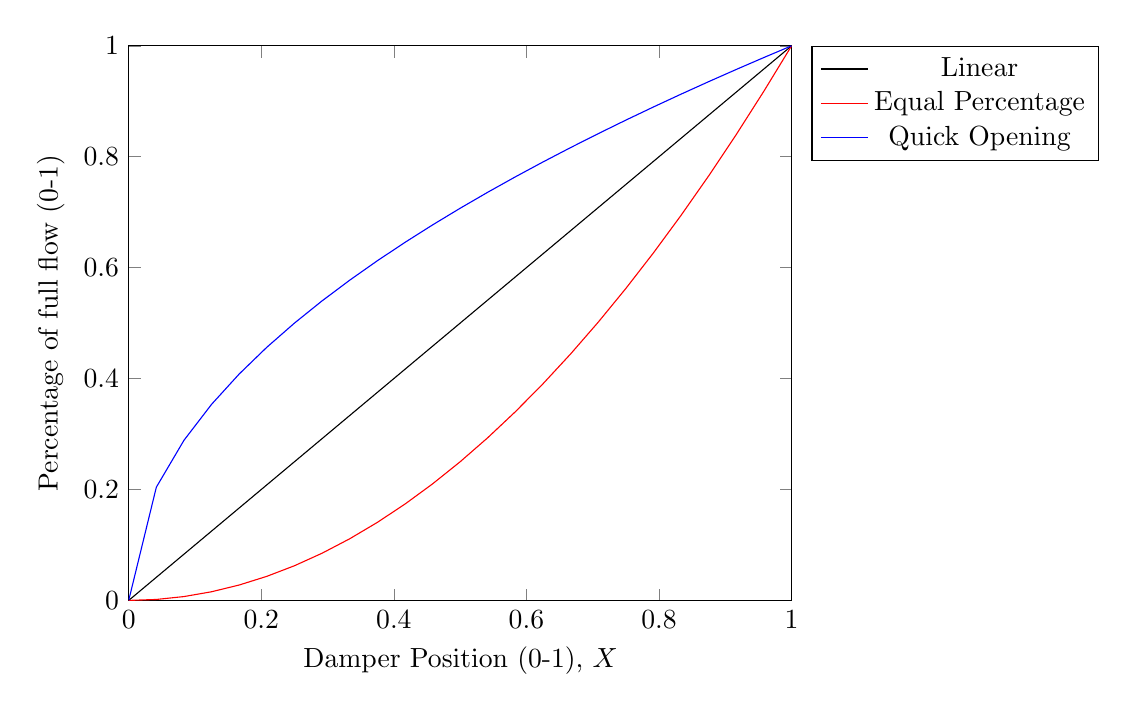
\begin{tikzpicture}

\begin{axis}[
        xmin=0,
        xmax=1,
        ymax=1,
        ymin=0,
        legend pos=outer north east,
        xlabel={Damper Position (0-1), \(\damp{}\)},
        ylabel={Percentage of full flow (0-1)},
    ] \addplot[
        domain=0:1,
        black,
    ]
    {x};

    \addlegendentry{Linear}

    \addplot[
        domain=0:1,
        red,
    ]{x*x};
    \addlegendentry{Equal Percentage}
\addplot[
        domain=0:1,
        blue,
    ]{sqrt(x)};
    \addlegendentry{Quick Opening}


\end{axis}



\end{tikzpicture}
\caption{Terminal box flow response as a function of damper position.}
\label{fig:flowVersusDamperPos}
\end{figure}


\section{Predicting the Mixed Air Temperature}

In order to predict the energy use at the cooling/reheat coils in the air handling unit, the mixed air temperature needs to be estimated. The mixed air temperature will be dependent on several variables including the outdoor air temperature, return air temperature, and the damper positions of the outdoor air and return air. The damper positions will fluctuate greatly during times of economizing.  

If the flow for both outside and return air are known, along with either estimates or measurements of \(\oat{}\) and \(\rat{}\), then \(\mat{}\) can be predicted directly using a straightforward energy balance. 

\begin{equation}
    \mat{} = \frac{\flow{oa} \oat{} + \flow{ra} \rat{}}{\flow{oa}+\flow{ra}}
\end{equation}

In many cases, the temperatures can be estimated, but the individual flows are not measured or are difficult to measure. In these cases, it makes sense to investigate \(\mat{}\) as a function of \(\oat{}\). If the system is constant volume, then the \(\mat\) will be linearly related to \(\oat\) and the coefficients in a linear regression will be equal to

\begin{equation}
    \mat = \left(  \frac{\flow{oa}}{\flow{tot}}\right) \oat + \frac{\flow{ra}\rat}{\flow{tot}}
\end{equation}

If economizing is programmed, there should be a significant moderation that should be present in \(\mat{}\).

In many cases, \(\mat\) will not vary significantly in operation and can be considered constant. The data can be investigated on a case-by-case basis and the best model of these can be used to estimate \(\mat\).

A robust approach that will be investigated is the \textit{nearest neighbor} approach. It is known that \(\mat\) is related to outdoor air temperature, return air temperature, along with the available damper positions in the particular air handler. By searching through historical data for similar conditions and taking the median of the data, a robust and reliable estimate can be made. 

Unfortunately, for a given request, only the outdoor air conditions and the time of day will be known. 


\section{Searching for Energy Minimum}

The fan power can be estimated using a fan curve as a function of the part load ratio (PLR) calculated using air flow rate. A fan curve suggested by Kimla that accounts for VSDs and constant static pressure setpoints is
\begin{equation}\label{eq:KimlaFanPower}
\frac{\dot{W}}{\dot{W}_{rated}} = 0.0013+0.147\left(PLR \right)+0.9506\left(PLR \right)^2-0.0998\left(PLR \right)^3
\end{equation}
where \(PLR\) is defined as \(\frac{\flow{}}{\flow{\text{design}}}\).

Since we are going to be using the gradient of this function, it is desired to reduce the order to the polynomial from 3 to 2. The corresponding closest second order polynomial to \ref{eq:KimlaFanPower} is
\begin{equation}\label{eq:finalFanPower}
\frac{\dot{W}}{\dot{W}_{rated}} = 0.21\left(PLR \right)+0.8\left(PLR \right)^2
\end{equation}

The total energy is the combination of fan, cooling, and reheat energy. If there are \(n\) terminal units, the total energy can be written as
\begin{multline}\label{eq:totalEnergy}
    \energy=\dot{W}_{rated}\;0.8 \left(\frac{\flowsum}{\flow{\text{design}}} \right)^2 + \dot{W}_{rated}\;0.21 \left(\frac{\flowsum}{\dot{V}_{design}} \right)\\
+1.08\left(\flowsum \right)\left(T_{ma}-T_{sa} \right)\\
+1.08\left(\flow{1} \right)\left(T_{z,1}-\frac{\dot{Q}}{1.08\; \flow{1}} -T_{sa}\right) +1.08\left(\flow{2} \right)\left(T_{z,2}-\frac{\dot{Q}}{1.08\; \flow{2}} -T_{sa}\right)\\ 
+\ldots+1.08\left(\flow{n} \right)\left(T_{z,n}-\frac{\dot{Q}}{1.08\; \flow{n}} -T_{sa}\right) 
\end{multline}
The first line is related to the fan energy, the second line is related to the cooling load at the air handling unit, and the last two lines relate to reheat energy use. 
This function \ref{eq:totalEnergy} is minimized under the constraints
\begin{align}
    V_{min}&\leq \flow{1}, \flow{2}, \ldots \flow{n} \\
T_{sa,min}&\leq T_{sa} \leq T_{sa,max} \\
    \sum_i^n \flow{i} &= V_T \leq V_{T,design} \\
\forall i\in\left\{1,\ldots,n\right\}: T_{dis,i} &= T_{z,i} - \frac{\dot{Q}_i}{1.08\;V_i} \geq T_{sa}
\end{align}

The partial derivatives of \ref{eq:totalEnergy} are 
\begin{multline}
    \pdv{\dot{E}}{V_i}=\frac{\dot{W}_{design}\;1.6}{\flow{design}^2} \left(\flowsum \right)\\ 
    +\frac{0.2\;\dot{W}_{design}}{\dot{V}_{design}}+ 1.08\left(\mat+T_{z,i} -2T_{sa}\right)
\end{multline}
\begin{equation}
    \pdv{\dot{E}}{\sat}=-2.16\left(\flowsum \right)
\end{equation}

\subsection{Brute Force Approach}

Since the system is not going to expected to determine semi-optimal control setpoints at small time intervals, say less than a second, it is plausible that a straightforward, brute force approach would be appropriate.
The brute force approach has several advantages including
\begin{enumerate}
        \item Straightforward to program and debug
        \item Robust to small changes in energy prediciton algorithm 
\end{enumerate}

The uncertainty in the estimation of the zone loads, plenum temperatures, mixed air temperature, and the like, also tend to support the decision to use step sizes on the order of  \SI{0.1}{\degreeF}. The typical search range for the supply air temperature will be on the order of \SI{20}{\degreeF}, making for a total number of calculations in the hundreds. 
This is extremely feasible for modern computers to handle in the sub-second time range. 

The minimum value of \(\sat\) in the search range would be the lowest feasible \(\sat\) possible dependent on the chilled water system and capacity of the cooling coils. 
This may be on the order of \SI{50}{\degreeF}.

The upper end of the search range will be the minimum of the \(\mat\) and the determined \(\dat\)'s.

\begin{equation}
    T_{sa,max} = \text{MIN}\left(\mat, \text{MIN}\left(T_{dis,1}, T_{dis,2}, \ldots, T_{dis,n} \right) \right)
\end{equation}

With a given zone load and constant flow, the \(\dat\) from the terminal unit can be calculated 
\begin{equation}
    \dat = T_{z} -  \frac{Q_{zone}}{1.08 \left( \text{CFM} \right)   }
\end{equation}
The primary airflow is then calculated from
\begin{equation}
    \flow{pri, req} = \totflow \left( \frac{T_{plen} - \dat }{T_{plen} - \sat} \right) 
\end{equation}
The actual primary airflow is then 
\begin{equation}
    \flow{pri} = \text{MAX}\left(\flow{pri, req}, \flow{pri, min}  \right)
\end{equation}

\section{Determining the Supply Air Static Pressure Requirement}

As shown in Section \ref{sec:FanModeling}, building up a complete air flow model is challenging. A different approach is to reduce the number of parameters by focusing on the \textit{critical zone}. 

One method of determining the critical zone is to simply check the percentage of time that a particular damper is the most open. This check can occur over any period, for example, over the previous week, month, or 6 months.

At a particular static pressure, there should exist some relationship between the damper position and the flow through the terminal unit. For a conservative estimate of the maximum flow at a given static pressure, the measured values of flow at the 90\% open damper position can be investigated. 

In a live setting, if data does not exist for a particular static pressure setpoint, then the system can slowly begin to explore until the desired number of data points are available. For example, the system could reduce the static pressure setpoint in increments of 0.1'' w.g. 




%\begin{sidewaysfigure}
%\begin{tikzpicture}
%
%\coordinate (bottomLeft) at (0,0);
%\coordinate (belowFan) at (0,5); 
%\coordinate (bottomRight) at (10,0);
%\coordinate (topLeft) at (0,13);
%
%\node [circle, draw] at (-2,10) {\(P_{s,fan}\) };
%
%\draw (bottomRight) -- (bottomLeft) -- (belowFan);
%\draw (-0.5,10) -- (0.5,10);
%\draw (-1, 10.5) -- (1,10.5);
%\draw (0,10.5) -- (topLeft);
%
%
%
%
%
%\end{tikzpicture}
%\end{sidewaysfigure}

\section{Handling of the Ramp Function}

In many cases related to steady state algorithms for determining the energy use of an air handling unit, ramp functions are found. These ramp functions are usually difficult to deal with in optimization problems because they are not continuously differentiable. In this sense, it is desired to have a replacement or approximation to the function that is smooth and can be differentiated. 

Fourier series are a useful tool for approximating arbitrary functions and can be used in this task. We can begin by focusing on the basic ramp function that is defined by:

\begin{equation}
f(x)=\begin{cases}0  & x < 0 \\
                  x  & x \geq 0
\end{cases}
\end{equation}

If we define our Fourier series to be defined over the interval \(-L \leq x \leq L\) and be equal to 

\begin{equation}
    f(x) = a_0 + \sum_{n=1}^\infty a_n \cos{\frac{n \pi x }{L}} + \sum_{n=1}^\infty b_n \sin{\frac{n \pi x }{L}}
\end{equation}

The coefficients are equal to

\begin{equation}
    a_0 = \frac{1}{2 L } \int_{-L}^{L} f(x) \; dx 
\end{equation}


\begin{equation}
    a_n = \frac{1}{L} \int_{-L}^{L} f(x) \cos{\frac{n \pi x}{L}} \; dx 
\end{equation}

\begin{equation}
    b_n = \frac{1}{L} \int_{-L}^{L} f(x) \sin{\frac{n \pi x}{L}} \; dx 
\end{equation}

\(f(x)=0\) when \(x \leq 0\), so that portion of the integral is equal to 0. When \(x \geq 0\), \(f(x)=x\) and the coefficients can be evaluated over the range \(0 \leq x \leq L\).

\begin{equation}
    a_0 = \frac{1}{2 L } \int_{0}^{L} x \; dx 
\end{equation}


\begin{equation}
    a_n = \frac{1}{L} \int_{0}^{L} x \cos{\frac{n \pi x}{L}} \; dx 
\end{equation}

\begin{equation}
    b_n = \frac{1}{L} \int_{0}^{L} x \sin{\frac{n \pi x}{L}} \; dx 
\end{equation}


Solving for \(a_0\), 

\begin{equation}
    a_0 = \frac{1}{2 L } \int_{0}^{L} x \; dx = \frac{1}{2 L} \left[ \frac{x^2}{2} \right]^{L}_{0} = \frac{1}{2 L} \left(\frac{L^2}{2} \right) = \frac{L}{4}
\end{equation}

The coefficients for the cosine terms are 

\begin{equation}
    \begin{split} 
        a_n &= \frac{1}{L} \int_{0}^{L} x \cos{\frac{n \pi x}{L}} \; dx \\ 
            &=  \frac{1}{L} \left(\cancelto{0}{x \frac{L}{n \pi}   \sin{\frac{n \pi x}{L}}  \bigg|^{L}_0}  - \int_0^L \frac{L}{n \pi} \sin{\frac{n \pi}{L} x} \; dx  \right) \\
            &= \frac{1}{L} \left( \left[ \frac{L^2}{n^2 \pi^2} \cos{\frac{n \pi x}{L}}  \right]^L_0 \right) \\
            &= \frac{L}{n^2 \pi^2}\left( (-1)^n - 1 \right)
    \end{split}
\end{equation}


and the coefficients for the sine terms are 


\begin{equation}
    \begin{split} 
        b_n &= \frac{1}{L} \int_{0}^{L} x \sin{\frac{n \pi x}{L}} \; dx \\ 
            &=  \frac{1}{L} \left(-x \frac{L}{n \pi}   \cos{\frac{n \pi x}{L}}  \bigg|^{L}_0  - \int_0^L -\frac{L}{n \pi}\cos{\frac{n \pi}{L} x} \; dx  \right) \\
            &= \frac{1}{L} \left( \left[ \frac{-L^2}{n \pi} (-1)^n  +\frac{L^2}{n^2 \pi^2}   \left[ \sin{\frac{n \pi x}{L}} \right]_0^L  \right] \right) \\
            &= \frac{1}{L} \left( \left[ \frac{-L^2}{n \pi} (-1)^n  + 0 \right] \right) \\
            &= \frac{L}{n \pi}\left( (-1)^{n+1} \right)
    \end{split}
\end{equation}


\chapter{\uppercase{NCTM Case Study}}
The National Center for Therapeutic Medicine (NCTM) was used as a test bed for the original methodology. NCTM is a building located on the campus of Texas A\&M University, in College Station, Texas. 

The National Center for Therapeutics Manufacturing (NCTM) combines the educational and manufacturing focuses of the biopharmaceutical industry. The NCTM building is approximately 150,000 ft\textsuperscript{2} with nearly 50,000 ft\textsuperscript{2} of educational facilities that include wet labs, culture facilities, large lecture halls, and a mock current Good Manufacturing Practice (cGMP) training suite. Around 120,000 ft\textsuperscript{2} is on the first level and 30,000 ft\textsuperscript{2} is on the second level. 

The cGMP Suite contains modern biopharmaceutical manufacturing equipment that students can use to learn industry practices. The wet labs are equipped with chemical fume hoods and the necessary electronic equipment for following standard operating procedures used in the biopharmaceutical industry. The lecture halls seat up to 120 students and have large floor to ceiling windows. There is also an Apple Computer laboratory with 48 workstations on the second floor. 

On the academic side there are three dedicated outdoor air handling units that serve seven child air handling units. Two of the air handling units are constant speed and the others are variable air volume. OAHU 1-1 serves its own wet lab and also feeds into AHU 1-1 and AHU 1-2. OAHU 1-2 serves AHU 1-3 and 1-4 on the first floor. OAHU 2-1 serves three children air handlers on the second floor, AHU 2-1, 2-2, and 2-3. 

This document focuses on the academic side of the building since Utilities and Energy services with Texas A\&M University are only allowed to make immediate changes to the HVAC system on this side. In summary, the important parameters concerning NCTM are that it houses several biopharmaceutical labs, it has an academic side that can be immediately changed and a manufacturing side that cannot be immediately changed, and relies on dedicated outdoor air handling units to pretreat outdoor air. 

\begin{table}
\centering
\begin{tabular}{l c c c}
\toprule
Level 			& OAHU	 	& AHU \# 	& AHU Schedule 		 \\
\midrule
Floor 1 Area B	& OAHU 1-1  & N/A		& 24/7 	 \\
Floor 1 Area B 	& OAHU 1-1 	& AHU 1-1	& 24/7 	 \\
Floor 1 Area B 	& OAHU 1-1	& AHU 1-2	& 6am - 6pm, M-F 	 \\
Floor 1 Area A 	& OAHU 1-2 	& AHU 1-3	& 6am - 8pm, M-F	 \\
Floor 1 Area A 	& OAHU 1-2	& AHU 1-4	& 6am - 8pm, M-F 	 \\
Floor 2 		& OAHU 2-1	& AHU 2-1	& 6am - 10pm, M-F 	 \\
Floor 2 		& OAHU 2-1 	& AHU 2-2	& 6am - 10pm, M-F	 \\
Floor 2			& OAHU 2-1	& AHU 2-3	& 6am - 10pm, M-F 	 \\
\bottomrule
\end{tabular}
\caption{Occupied/Unoccupied scheduling for the AHUs as described.}
\label{tab:OnOffSched}
\end{table}


\begin{figure}
    \centering
\includegraphics[]{Plots/TempRiseVsFlow-AHU-2-14.pdf}
\caption{Temperature rise due to the mixing of plenum air at the terminal box for FPVAV-2-14. }
\end{figure}

\begin{table}
\centering
\begin{tabular}{l c c}
\toprule
OAHU & Design OA CFM & HP \\
\midrule
OAHU 1-1 & 12,800 & 20 \\
OAHU 1-2 & 4,500 & 5 \\
OAHU 2-1 & 2,200 & 2 \\
\bottomrule
\multicolumn{1}{r}{Total:} & 19,500 & 27 \\
\end{tabular}
\caption{Fan schedule information for the dedicated outdoor air handlers.}
\label{tab:OAFanSched}
\end{table}

\begin{table}
\centering
\begin{tabular}{l c c c c}
\toprule
AHU 	& Type	 	& Total Airflow (CFM) 	& HP 	& OA Served By\\
\midrule
AHU 1-1 & Constant  & 3,000 			  	& 5 	& OAHU 1-1 \\
AHU 1-2 & VAV 		& 4,800 				& 5 	& OAHU 1-1 \\
AHU 1-3 & VAV 		& 7,500 				& 7.5 	& OAHU 1-2 \\
AHU 1-4 & Constant 	& 5,000 				& 7.5 	& OAHU 1-2 \\
AHU 2-1 & VAV 		& 6,000 				& 7.5 	& OAHU 2-1 \\
AHU 2-2 & VAV		& 8.500					& 10 	& OAHU 2-1 \\
AHU 2-3 & VAV 		& 6,000					& 7.5	& OAHU 2-1 \\
\bottomrule
\multicolumn{2}{r}{Total:} & 40,800 & 50 &  \\
\end{tabular}
\caption{Fan schedule information for the AHUs.}
\label{tab:FanSched}
\end{table}

\section{Terminal Unit Information}

On the academic side, there are a total of 10 series fan powered terminal units on the first floor and 18 on the second floor. 


\section{Analysis of Zone Load Predictions}

An important factor in the optimization methodology is the prediction of the zone loads at a given time, without access to current live sensor information. 

Before analyzing the prediction ability of different zone loads, it is important to gather insight into the nature of the calculated variable that is proposed to be used as the surrogate for zone load.   

If the zone loads are being met and steady-state conditions are assumed, the sensible zone load will be

\begin{equation}
    Q_{zone}=\flow{z} \rhocp{} \left(T_{dis}-T_{z} \right) \approx 1.1 \cdot \flow{z}\left(T_{dis}-T_{z} \right)
\end{equation}

A useful simplification would be replacing the \(\rhocp{}\) term with a constant value. A value of 1.1, when \(\flow{z}\) is in units of CFM and temperature is in units of \(^\circ\)F is common. 

\section{Analysis of the Mixed Air Temperature and Reheat Assumption}

For series fan powered boxes, the assumption was made that the total flow remains constant and that the mixed air temperature at the individual box can be predicted based on the primary flow value that is measured. 


\section{Analysis of the Critical Zone Assumption}

The critical zone/damper is to be used to determine the static pressure setpoint that can be used to supply the desired flows found from the optimization. An important consideration in the methodology is checking how how this assumption holds. Data from NCTM can be used to test the validity of the approach.




%%%%%%%%%%%%%%%%%%%%%%%%%%%%%%%%%%%%%%%%%%%%%%%%%%%%%%%%%%%%%
\let\oldbibitem\bibitem
\renewcommand{\bibitem}{\setlength{\itemsep}{0pt}\oldbibitem}
%%%%%%%%%%%%%%%%%%%%%%%%%%%%%%%%%%%%%%%%%%%%%%%%%%%%%%%%%%%%%%%
\include{bibliography}
% \include{appendices}


\end{document}
